% !TeX root = ../main.tex
\section{Evaluation}
\label{sec:evaluation}
\raggedbottom




\subsection{Experimental Setup}
\textbf{Hardware.}
The A100 experiments use one NVIDIA A100 80~GB PCIe GPU and an HDD RAID backing store.
The large-model experiment uses one NVIDIA H100 SXM 80~GB GPU with 3.35~TB/s HBM3 bandwidth and a PCIe Gen5 host link.
Its HDD RAID sustains about 425~MiB/s sequential reads.
Expert weights remain in FP16 throughout.

\textbf{Models and workloads.}
A100 runs cover Mixtral-8$\times$7B and Qwen2-57B-A14B on WikiText-2, GSM8K, and HumanEval.
The H100 run uses the 141B-parameter Mixtral-8$\times$22B-Instruct-v0.1 with 56 layers, eight experts per layer, and top-2 routing.
Each expert occupies 576~MiB, yielding about 252~GiB of FP16 expert weights.

\textbf{Baselines.}
The A100 comparison includes on-demand Streaming, Fiddler, MoE-CORE, MoE-Infinity, SSD-LLaMA, and FlashMoE-RF~\cite{fiddler,core,moeinfinity,ssdllama,flashmoe}.
The H100 comparison includes Streaming, Fiddler, FlashMoE-RF, and MECC.
Streaming loads each requested expert from the backing store when it is needed.

\textbf{Metrics.}
TTFT measures time to the first token; TPOT averages the time per subsequent token.
Both include computation and expert delivery, and we average latency across prompts.
Figure~\ref{fig:performance} reports $T_{\mathrm{Fiddler}}/T_{\mathrm{method}}$ for each model, workload, and metric; values above one indicate lower latency than Fiddler.
Figure~\ref{fig:h100_main} uses the same ratio for H100.

\subsection{End-to-End Performance}
\begin{figure}[H]
\centering
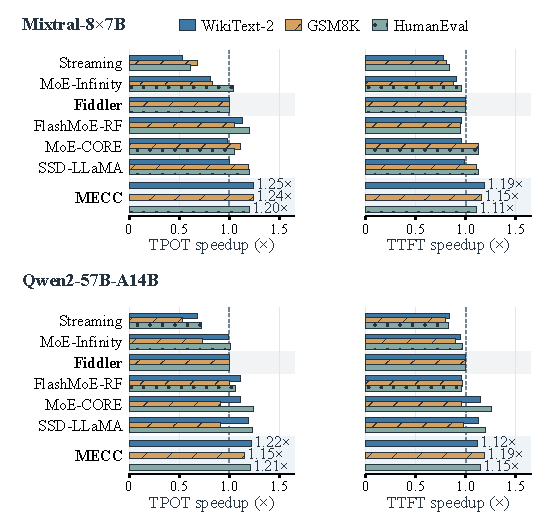
\includegraphics[width=\columnwidth]{figures/fig08_a100_singlecolumn.pdf}
\caption{A100 TPOT and TTFT speedup over Fiddler for Mixtral-8$\times$7B and Qwen2-57B-A14B. MECC values appear beside the bars; higher is better.}
\label{fig:performance}
\end{figure}
Figure~\ref{fig:performance} compares the two A100 models on three tasks. Relative to Fiddler, MECC reaches 1.20--1.25$\times$ TPOT and 1.11--1.19$\times$ TTFT speedup on Mixtral-8$\times$7B, and 1.15--1.22$\times$ TPOT and 1.12--1.19$\times$ TTFT speedup on Qwen2-57B-A14B. It improves both metrics on all six model--task pairs. Mixtral's TPOT range is narrow, while Qwen2 GSM8K has its smallest TPOT gain and largest TTFT gain.
TTFT includes initial expert accesses, when the request has had little opportunity to build a resident working set. TPOT also captures later revisits after experts have moved between HBM and CPU. These access windows help explain why the workload order differs across the two metrics.

The baselines address different parts of the path. MoE-CORE allocates GPU slots across layers from domain-level routing statistics~\cite{core}; SSD-LLaMA updates RAM and VRAM caches using access history~\cite{ssdllama}. MoE-Infinity uses routing traces for replacement and prefetching~\cite{moeinfinity}, and FlashMoE-RF uses recency and frequency for eviction~\cite{flashmoe}. MECC allocates both HBM and CPU slots across layers, starts their resident lists at distinct cuts, and reuses a released CPU slot when a host expert is promoted. This keeps a displaced GPU expert available for later requests without a device-to-host copy.

TTFT reflects cold first touches before reuse develops. MECC seeds residency from offline routing counts and has TTFT bars above one for every pair. On Qwen2 GSM8K, its TPOT and TTFT bars reach 1.15$\times$ and 1.19$\times$. For each model, the geometric mean across bars places MECC 6--8\% ahead of SSD-LLaMA, the second-best method.

\begin{figure}[H]
\centering
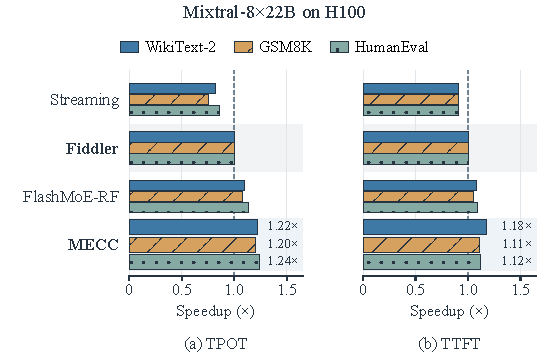
\includegraphics[width=\columnwidth]{figures/fig09_h100_main.pdf}
\par\nointerlineskip
\caption{H100 TPOT and TTFT speedup over Fiddler for Mixtral-8$\times$22B-Instruct-v0.1 across three tasks (128/128 tokens). Colors follow Figure~\ref{fig:performance}; higher is better.}
\label{fig:h100_main}
\end{figure}

Figure~\ref{fig:h100_main} examines Mixtral-8$\times$22B in the HDD-backed setup. Across WikiText-2, GSM8K, and HumanEval, MECC reaches 1.20--1.24$\times$ TPOT and 1.11--1.18$\times$ TTFT speedup over Fiddler. FlashMoE-RF reaches 1.08--1.14$\times$ and 1.05--1.09$\times$; Streaming reaches 0.75--0.86 of Fiddler on TPOT. MECC leads on both metrics for all three tasks. A changed top-2 pair can still trigger an HDD read; retaining a displaced expert in host memory reduces the cost of a later revisit.

\subsection{Mechanism Analysis}
We measure component additions and task transfer.
\begin{figure}[H]
\centering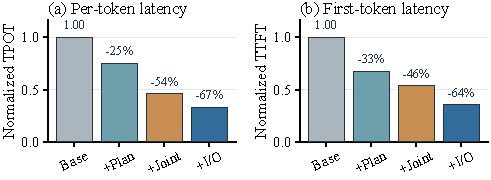
\includegraphics[width=\columnwidth]{figures/fig09_ablation_startup.pdf}
\par\nointerlineskip
\caption{Component sequence: (a) TPOT and (b) TTFT normalized to Base.}
\label{fig:ablation_components}
\end{figure}
\textbf{Component addition.} Base fills each layer's HBM and CPU slots in expert-ID order, replaces the two resident sets independently without admitting HBM victims to CPU, and serves non-HBM experts serially, reading HDD on a double miss before H2D. The stages share HBM/CPU budgets, requests, and FP16 weights. In Figure~\ref{fig:ablation_components}, +Plan changes initial residents to routing-count ranks; +Joint links promotion to CPU admission and reuses displaced experts' host copies; +I/O overlaps selected HDD reads with resident work and batches eligible CPU-resident transfers. TPOT falls to 0.75, 0.46, and 0.33; retention gives the largest decoding step by preserving displaced experts in CPU. TTFT falls to 0.67, 0.54, and 0.36; placement gives the largest first-token step by reducing HDD-served requests from 84\% to 56\%. The placement step acts before later accesses have populated the cache, while joint retention has more opportunities during decoding.


\begin{figure}[H]
\centering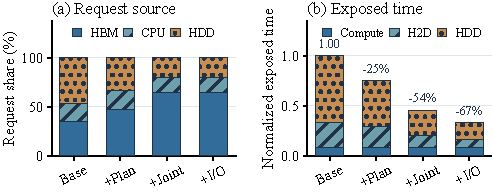
\includegraphics[width=\columnwidth]{figures/fig10_traffic_exposure.pdf}
\par\nointerlineskip
\caption{Component sequence: (a) expert request sources and (b) exposed time normalized to Base.}
\label{fig:ablation_traffic}
\end{figure}
\textbf{Traffic and delivery.} Figure~\ref{fig:ablation_traffic} separates where expert weights are found from how long delivery delays execution. Retention can turn a later HDD read into a CPU hit, changing request-source fractions. Delivery reduces exposed time from 0.46 to 0.33 of Base without changing those fractions. The source panel counts every request, including one whose read overlaps computation; the time panel counts only delay left on the execution path. During prefill, a pending read may overlap work on an HBM-resident expert. These two views show different effects of caching and scheduling.

\begin{figure}[H]
\centering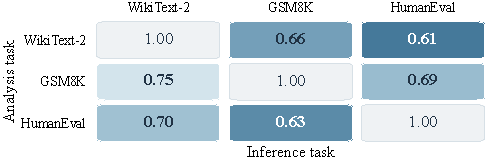
\includegraphics[width=\columnwidth]{figures/fig15_profile_mismatch.pdf}
\par\nointerlineskip
\caption{Task transfer. Rows give analysis tasks and columns inference tasks. Cells show TPOT relative to fixed residency; lower is better.}
\label{fig:task_transfer}
\end{figure}
\textbf{Task transfer.} In Figure~\ref{fig:task_transfer}, online membership lowers mean TPOT to 0.67 of fixed residency across the six changed-task pairs; matched-task entries remain at one. The smallest off-diagonal entry in the HumanEval inference column is 0.61, the largest reduction across the matrix. Newly selected experts enter the resident hierarchy under the same slot budgets and can serve later requests. The diagonal cells provide a matched-task reference. For changed tasks, early accesses may still require a transfer; later requests can reuse the updated resident set.

\flushbottom
